\documentclass[a4paper]{article}

% natbib
\usepackage[numbers,sort]{natbib}

\usepackage{mysimpletemplatewn}
\usepackage[utf8]{inputenc} %%% to support copy and paste with accents for french stuff
\usepackage[T1]{fontenc} %%%key to get copy and paste for the code!
\usepackage{times}
\usepackage[french]{babel}
\usepackage[scaled=0.85]{helvet}
\usepackage{graphicx}
\usepackage{ifthen}
\usepackage{xspace}
\usepackage{alltt}
\usepackage{latexsym}
\usepackage{url}
\usepackage{amsmath,amssymb,amsfonts}
\usepackage{stmaryrd}
\usepackage{algorithmic}
\usepackage{textcomp}
\usepackage{xcolor}
\usepackage{enumerate}
% \usepackage{cite}
\usepackage[pdftex,colorlinks=true,pdfstartview=FitV,linkcolor=blue,citecolor=blue,urlcolor=blue]{hyperref}
\usepackage{multirow}
\usepackage{listings}
\usepackage{color}
\usepackage{subcaption}

\usepackage{pgfgantt}

\usepackage{bibentry}
\nobibliography*


\newboolean{showcomments}
\setboolean{showcomments}{true}
\ifthenelse{\boolean{showcomments}}
  {\newcommand{\bnote}[2]{
	\fbox{\bfseries\sffamily\scriptsize#1}
    {\sf\small$\blacktriangleright$\textit{#2}$\blacktriangleleft$}
    % \marginpar{\fbox{\bfseries\sffamily#1}}
   }
   \newcommand{\paragraphDesc}[2]{
    \textcolor{#1}{#2}
   }
   
  }
  {\newcommand{\bnote}[2]{}
   \newcommand{\cvsversion}{}
   \newcommand{\paragraphDesc}[2]{}
  }

\newcommand{\here}{\bnote{***}{CONTINUE HERE}}
\newcommand{\nb}[1]{\bnote{NB}{#1}}

\newcommand{\fix}[1]{\bnote{FIX}{#1}}
%%%% add your own macros 


\newcommand{\sd}[1]{\bnote{Stef}{\textcolor{orange}{#1}}}
\newcommand{\an}[1]{\bnote{Anne}{\textcolor{green}{#1}}}
\newcommand{\bv}[1]{\bnote{Benoit}{\textcolor{blue}{#1}}}
\newcommand{\nic}[1]{\bnote{Nic}{\textcolor{red}{#1}}}

\newcommand{\todo}[1]{\bnote{TODO}{#1}}

\graphicspath{{figures/}}
%%% 


\newcommand{\figref}[1]{Figure~\ref{fig:#1}}
\newcommand{\figlabel}[1]{\label{fig:#1}}
\newcommand{\tabref}[1]{Table~\ref{tab:#1}}
\newcommand{\layout}[1]{#1}
\newcommand{\commented}[1]{}
\newcommand{\secref}[1]{Section~\ref{sec:#1}}
\newcommand{\seclabel}[1]{\label{sec:#1}}

%\newcommand{\ct}[1]{\textsf{#1}}
\newcommand{\stCode}[1]{\textsf{#1}}
\newcommand{\stMethod}[1]{\textsf{#1}}
\newcommand{\sep}{\texttt{>>}\xspace}
\newcommand{\stAssoc}{\texttt{->}\xspace}

\newcommand{\stBar}{$\mid$}
\newcommand{\stSelector}{$\gg$}
\newcommand{\ret}{\^{}}
\newcommand{\msup}{$>$}
%\newcommand{\ret}{$\uparrow$\xspace}

\newcommand{\myparagraph}[1]{\noindent\textbf{#1.}}
\newcommand{\eg}{\emph{e.g.}\xspace}
\newcommand{\ie}{\emph{i.e.}\xspace}
\newcommand{\etal}{\emph{et al.,}\xspace}
\newcommand{\ct}[1]{{\textsf{#1}}\xspace}
\newcommand{\etc}[1]{\textit{etc.}}



\newcommand{\defaultScale}{0.55}
\newcommand{\pic}[3]{
   \begin{figure}[h]
   \begin{center}
   \includegraphics[scale=\defaultScale]{#1}
   \caption{#2}
   \label{#3}
   \end{center}
   \end{figure}
}


\newcommand{\twocolumnpic}[3]{
  \begin{figure*}[!ht]
  \begin{center}
  \includegraphics[scale=\defaultScale]{#1}
  \caption{#2}
  \label{#3}
  \end{center}
  \end{figure*}
}

\newcommand{\picw}[3]{
  \begin{figure}[htbp]
  \begin{center}
  \includegraphics[width=\columnwidth]{#1}
  \caption{#2}
  \label{#3}
  \end{center}
  \end{figure}
}


\newcommand{\infe}{$<$}
\newcommand{\supe}{$\rightarrow$\xspace}
\newcommand{\di}{$\gg$\xspace}
\newcommand{\adhoc}{\textit{ad-hoc}\xspace}

\usepackage{url}            
\makeatletter
\def\url@leostyle{%
  \@ifundefined{selectfont}{\def\UrlFont{\sf}}{\def\UrlFont{\small\sffamily}}}
\makeatother
% Now actually use the newly defined style.
\urlstyle{leo}

\definecolor{codegreen}{rgb}{0,0.6,0}
\definecolor{codegray}{rgb}{0.5,0.5,0.5}
\definecolor{codepurple}{rgb}{0.58,0,0.82}
\definecolor{backcolour}{rgb}{0.95,0.95,0.92}

\lstdefinestyle{mystyle}{
    backgroundcolor=\color{backcolour},
    commentstyle=\color{codegreen},
    keywordstyle=\color{magenta},
    numberstyle=\tiny\color{codegray},
    stringstyle=\color{codepurple},
    basicstyle=\footnotesize,
    breakatwhitespace=false,
    breaklines=true,
    captionpos=b,
    keepspaces=true,
    numbers=left,
    numbersep=5pt,
    showspaces=false,
    showstringspaces=false,
    showtabs=false,
    tabsize=2
}

\lstset{style=mystyle}
\newcommand{\browserMaster}{\textit{BrowserMaster} \xspace}

\title{CST --Analyse multi-facettes et opérationnelle pour la transformation des systèmes d’information}
\author{ HOUEKPETODJI Mahugnon Honoré}

\begin{document}

\institution{}

\date{\today}

\maketitle

% \begin{abstract}
% The abstract text goes here.
% \end{abstract}
\section{Description du sujet de la thèse}
% 0.5 (1/2) pages
CIM est une SAS au capital social de 200 000 euros détenu à 100\% par DL Software. 
CIM est éditeur, intégrateur, hébergeur et infogéreur de solutions pour l'assurance de personnes en santé, prévoyance. 
Elle offre une expertise Santé et Prévoyance acquise après plus de 30 ans auprès de ses clients. 
CIM est hébergeur de ses solutions pour 90\% de ses clients et plus de 1000 utilisateurs. 
Toutes les thématiques d'infrastructure et de surveillance des flux sont intégrées à cette offre.
CIM est propriétaire de ses infrastructures serveurs, tous les éléments actifs des systèmes et tous les éléments de stockage sont achetés par CIM, gérés et supervisés par les équipes de CIM. Aucun sous-traitant n'intervient dans les opérations quotidiennes d'hébergement, d'exploitation des solutions et des données hébergées.

CIM est certifiée \textit{Microsoft GOLD Partner}. 
Elle est l'éditeur des progiciels de la gamme Izy Links et assure l'intégration de l'ensemble des briques de cette gamme ainsi que des briques partenaires nécessaires à la bonne réussite du projet.
 Cette solution est développée en PowerBuilder sur une base de données DB2.
L'équipe de développement vient d'avoir PowerBuilder version 2017 (été 2018) et est en cours de passage sur DB2 v11.

Le système de gestion est centré sur Izy Protect, autour duquel gravite l'ensemble des briques complémentaires répondant à l'assemble des besoins, et pouvant être activées ou non. 
La société CIM a effectué une analyse de risque pour son évolution et croissance en 2017.
D'où il ressort que Izy Protect souffre des problèmes 
(1) vieux langage,
(2) logiciel vieillissant,
(3) perte de savoir,
(4) changements à haut risque.
Ces problèmes sont récurrents chez les organismes gérant des systèmes d'information \cite{Deme02a}.

Face à cette situation CIM souhaite entreprendre des actions en particulier migrer la partie métier d'Izy Protect vers \textit{C\#}.
Ce travail de doctorat consiste à proposer des modèles et des mécanismes d'aide pour une ré-ingénierie des systèmes d'information. 
Par exemple, des mécanismes et des outils permettant d'aider les développeurs  de la CIM à migrer la partie métier d'Izy Protect vers \textit{C\#}.
Les expériences et validation des prototypes se feront dans le contexte de l'application du système d'information écrit en PowerBuilder de la société CIM.


\section{Etat de l'art}
\label{sec:stateOfTheArt}
% 1 pages
Dans cette section, je presenterai Izy Protect et les travaux qui se penchent sur la question de la ré-ingénierie des systèmes d'information.
%===========================================================================================================================================================
\subsection{Présentation d'Izy Protect}
\label{sec:izyProtect}
Izy Protect est un système de plus de 3 millions de lignes de code écrites en PowerBuilder et maintenu depuis plus de 20 ans par les développeurs de la CIM. 
Aujourd'hui Izy Protect est maintenu par une équipe de 18 développeurs.
 Le code source est organisé par bibliothèques PowerBuilder. 
Izy Protect compte 117 bibliothèques. Les bibliothèques d'Izy Protect peuvent être regroupées en des modules métier.
 Par contre cette information ne peut pas être directement déduite du code.
 La plus large a une taille d'environ 300 000 lignes de code.
Durant toutes ces années, il y a eu beaucoup de changements dans l'équipe de développeurs. 
Vu la complexité actuelle du système, les développeurs ont de plus en plus du mal à le maintenir.
Les anciennes versions du système sont stockées sur un disque dur.
 Pour des raisons internes à la CIM, les versions d'Izy Protect ont été perdues jusqu'en 2010. 
 De plus, les développeurs risquent à tout moment de faire de régression (casser une fonctionnalité existante). 
Pour cause, le code source de Izy Protect  n'est pas couvert avec des tests unitaires automatisés.
Ceci augmente la craint des développeurs pour de petites modifications. 
Les caractéristiques d'Izy Protect montrent qu'il est un système qui a une grande valeur pour l'entreprise et 
 il est développé avec un vieux langage de programmation: PowerBuilder. 
Par conséquent, il est  \textbf{patrimonial} selon \citet{Deme02a}.
Quand un système a plusieurs décennies de vie, la rétro-ingénierie est une activité centrale pour le maintenir \cite{Deme02a}.

Dans l'entreprise, les travaux de maintenances ou de développements sur Izy Protect sont identifiés par des tickets.
Les tickets sont stockés dans la base de données des tickets ou fiches navettes depuis 1998. 
La base de données des tickets pilote l'ensemble du processus d'évolution du logiciel : attribution du travail aux développeurs, gestion du flux de travail pour répondre à une demande du client, informations de facturation sur chaque tâche.
Il existe des tickets pour la correction de défauts, la rédaction de documentation, l'ajout de nouvelles fonctionnalités, etc. 

Un ticket comporte entre autres les caractéristiques suivantes:

\begin{itemize}
\item la date de création
\item la date de clôture
\item l'estimation du temps nécessaire au développeur pour travailler sur le ticket
\item temps passé par un développeur
\begin{itemize}
\item le temps d'analyser
\item le temps de mettre en œuvre une solution
\item le temps de test
\end{itemize}
\item le(s) bibliothèque(s) impactée(es)
\end{itemize}

%Etat d'Izy protect et les tests
Izy Protect  est planifié pour les tests de régressions lorsque  les modifications concernent certaines parties du système présélectionnés par l'entreprise.
Il faut noté que ces parties sont statiques.
Les tests de régressions sont subdivisés en deux parties: les tests de traitements de données(tests fonctionels) et les tests IHMs.
Les tests de traitements de données et les test IHMs sont automatisés.
Les tests de données sont des tests \textit{black box}: on passe des données en entrée par \textit{Bash}, on suit l'exécution et on compare la sortie. 
Tandis que les tests IHMS sont fait avec l'outil Tosca \cite{tosca}. 
Par contre, au cas où les modifications concernent d'autres parties du système, il n'y a aucune assurance qu'il n'a  pas de régressions ce qui peut parfois se faire sentir chez le client.

\subsection{Les tests automatisés et le DevOps}
%Etat d'Izy protect et les tests

%Littérature
\citet{Dude12a}  ont étudié les avantages et les limitations de l'automatisation des tests.
Ils ressortent que  les tests automatisés sont  répétables et réutilisables.
Les tests automatisés assurent aussi une couverture du code et un gain de temps dans l'exécution des tests.
Mais en contrepartie, les tests automatisés coûtent pour la mise en place(sélection d'outil, achat de l'outil de tests, conception des cas de tests), formations du personnel.

\citet{Yuqi20a} ont présenté une étude qui examine le degré de maturité du processus d'automatisation des tests par rapport aux pratiques d'automatisation des tests adopter dans ces entreprises de logiciels.
Ils remarquent que la culture du DevOps favorise un haut degré de  maturité du processus d'automatisation des tests.

\citet{Jess20a} ont enquêté sur  pourquoi les entreprises installent la culture du DevOps  dans leurs organisations. 
Les résultats montrent que les entreprises avaient besoin de: être plus agile et rapide, répondre aux tendances du marché, livrer les produits\/services de meilleure qualité,
réduire le temps de configuration des environnements,  améliorer la communication entre les équipes, introduire le processus d'automatisation et amener les commerciaux, les développeurs, et les opérateurs à avoir un objectif fonctionel commun. 
L'installation du DevOps à apporter: une rapidité de livraison, une meilleure qualité des produits et services, automatisation des processus,
améliorer la collaboration et la communication entre les équipes et une meilleure concentration sur les besoins du client.



\subsection{Analyse de l'évolution de l'état d'un système logiciel patrimonial}
\label{sec:etatLogiciel}
Les systèmes patrimoniaux sont des systèmes en constant changement : production de nouvelles fonctionnalités.
La deuxième loi de Lehman \cite{Lehm96a} stipule qu'à mesure que les logiciels évoluent, la complexité croissante et l'augmentation des défauts entraîneront une baisse de la satisfaction des parties prenantes, à moins que les équipes de projet n'entreprennent le travail nécessaire pour maintenir la qualité.
Selon \citet{Deme02a}, collecter et interpréter les données et les résumer dans une vue cohérente est une étape importante pour la compréhension initiale d'un système logiciel existant.
Dans ce sens, de nombreux travaux de la littérature proposent des techniques, pour suivre l'évolution de l'état de ces systèmes.

\citet{Zhan10b} utilise les données des occurrences bugs et le temps pour modéliser l'évolution d'un système logiciel avec c\-charts.

\citet{lenar17} propose un système de recommandation d'action au développeur pour un nouveau bug.
Le système se base sur l'historique des bugs, le code source ainsi que qu'un algorithme de prédiction.
Pour que ça marche, le code source doit être géré dans un système de contrôle de versions. 
Ce qui n'est pas le cas avec Izy Protect.

\citet{port17} utilise les modèles et l'analyse de l'historique des défauts pour évaluer la qualité d'un système et prédire l'effort nécessaire pour améliorer le système. Les métriques mesurées sont : le taux de bugs sur une période de temps, le ratio entre le taux d'augmentation de la taille du système et le taux de bugs, le temps moyen entre la découverte des bugs, l'effort pour résoudre les bugs, estimation des risques de futurs bugs...
Certain de ces métriques comme : le taux de bugs par période de temps, l'effort pour résoudre les bugs sont intéressants dans le cadre d'Izy Protect. 
Les autres ne se conforment pas au contexte, car les tickets d'Izy protect ne sont pas directement liés au code de façon standard.
Chaque développeur note le numéro de tickets à sa façon dans le code. 


\citet{kim07,Bibi06} proposent des modèles de prédiction des défauts avec des algorithmes d'apprentissage en utilisant l'historique des bugs de système. 
Les algorithmes de prédiction de bugs ne sont pas toujours consistants \cite{bang19}. De plus, ils ne tiennent pas compte des changements qui peuvent être imprévisible dans le code. 
En plus, Izy Protect est logiciel commercial, multi-utilisateur, et donc chaque utilisateur a des fonctionnalités ou des changements qui lui sont spécifiques. 

\citet{naga05} utilise l'historique le nombre de lignes de code changées pour une correction de  bug  ou une nouvelle fonctionnalité pour prédire la densité de bug dans le code.
 Pour que ceci soit réalisable, il faut que le code soit préalablement versionné dans un système de contrôle de versions.

\citet{Raja09} a étudié différents algorithmes de modélisation des défauts d'un système à partir des données des défauts relevés sur huit projets dont les codes sources sont ouverts. Il en ressort que la moyenne glissée modélise mieux les défauts des systèmes.

\subsection{Rétro-ingénierie}
\label{sec:retroingenierie}
Dans cette section, je présenterai les travaux reliés à l'outillage pour la rétro-ingénierie que j'ai étudiée.
\citet{Chik90a} définissent la rétro-ingénierie comme \textit{un processus d'analyse d'un système donné pour identifier les composants du système et leurs relations, afin de créer des représentations du système sous une autre forme ou à un niveau d'abstraction plus élevé."}.

\citet{Brun14c} affirment que la rétro-ingénierie n'est pas limitée à certains langages courants, mais est universelle. 
Par exemple, elle peut concerner la base de données \cite{Delp20a} ou l'interface graphique \cite{Verh19a}.
Il est donc nécessaire de disposer d'une suite d'outils polyvalents et extensibles, indépendants du langage : cette extension peut se faire à plusieurs niveaux - métamodèle, mais aussi au niveau des outils eux-mêmes (par exemple en agissant sur le modèle).

C'est dans cette optique que \citet{Kien10a} énoncent la retro-ingénierie nécessite des outils qui fournissent des fonctionnalités permettant d'extraire des informations de bas niveau des systèmes, d'analyser et de générer des connaissances sur les systèmes, et de visualiser ces connaissances afin que les ingénieurs puissent comprendre efficacement les aspects du système qui les intéressent.
De ce point de vue ils identifient que ces outils doivent être:

  (1) scalable: capacité de ces outils à s'adapter au changement de taille du logiciel;
  (2) interoperable: ces outils doivent être capable de communiquer avec des outils externes;
 (3) personnalisable: les activités de rétro-ingénierie étant variables, les utilisateurs d'outils de rétro-ingénierie doivent pouvoir continuellement
 les  adapter pour répondre aux besoins changeants;
 (4) utilisable: facilité d'utilisation;
(5) adoptable: facilité d'apprentissage.


\citet{Bell98a} ont proposé un ensemble de critères pour comparer les outils de rétro-ingénierie.
Par contre, ils ne couvrent pas le métamodèle, l'extension du métamodèle et des outils de manière exhaustive.

\citet{Govi18a} ont identifié des critères pour les outils de réingénierie. 
Parmi ces critères, j'ai retenu ceux qui se rapportent à la rétro-ingénierie.
Ce sont les critères (1) de sélection (2) d'abstraction.  
Le critère de sélection exige que l'outil de rétro-ingénierie permette à l'utilisateur de sélectionner des éléments  du code source d'un système 
qui répondent à une requête donnée.
L'outil doit aussi permettre à l'utilisateur d'abstraire les caractéristiques des entités du code source à un haut niveau d'abstraction. 
Par exemple: déduire de la complexité cyclomatique des classes d'un package, la complexité cyclomatique du package.



%Modisco
\citet{Brun14c} ont proposé et mis en œuvre le cadre MoDisco.
MoDisco est divisé en 4 couches, un projet de modélisation de la plateforme Eclipse, l'infrastructure, la technologie et les cas d'utilisation.
La couche infrastructure contient des outils génériques permettant de naviguer et d'interroger les modèles.
La couche technologie contient le métamodèle spécifique (Java, XML, JSP, ...).
Et la couche des cas d'utilisation contient l'action spécifique pour un modèle, par exemple le remaniement de code Java.
MoDisco inclut: un navigateur de modèle, un éditeur pour voir le code des entités d'un modèle, un support graphique pour faire des requêtes sur les éléments du modèle. 
Par contre \citet{Brun14c}, ne propose que l'UML pour visualiser les éléments d'un modèle.
Alors que pour  un logiciel patrimonial, Izy Protect par exemple, l'UML devient vite une toile d'araignée et freine une compréhension rapide du système.

%===============================================================================================================================================================
\section{Avancées actuelles}
% 3 pages
\subsection{Route vers le DevOps}
\label{sec: devOps}

Izy Protect présente les problèmes cités dans la \secref{izyProtect} en particulier, code non versionné, ce qui engendre les pertes et écrasement de code, puis l'absence totale de tests uintaires automatisés qui couvrent les fonctionnalités au niveaux du code source, etc.
Mon objectif est de construire des outils visant à aider  à la réingénierie de Izy Protect. 

Par ailleur, \citet{Deme02a} affiment que les tests sont comme une assurance de vie dans le cadre de la réingénierie logicielle. 
Ils vont plus loin pour dire que les tests permettent de garantir les activités de réingénieries ne vont pas modifier la logique metier.  
Sachant que la réingénierie de Izy Protect se fera de façon incrémentale, en cas d'erreur, il est important de savoir quel changement a cassé le code.
Un système de contrôle de versions et les tests automatisés seront d'une grande utilité pour les activités de réingénieries.
De plus, le fait de versionner le code  non seulement permet d'éviter les problèmes de pertes de code mais aussi à long terme me permettra aussi 
d'avoir une base d'analyse de l'évolution du code d'Izy Protect suplémentaire et de fournir  un outil de vérification des normes de développements sur les changements effectués par les développeurs.

J'ai choisi Subversion (SVN) \cite{svn} par le fait de sa simplicité pour la compréhension.
Il faut aussi noté que le module de contrôle de versions qu'offre PowerBuilder n'est pas trop stable. 
Par exemple, parfois, le module considère un code déjà versionné comme un code non versionné.
De plus, le module de contrôle de versions qu'offre PowerBuilder ne supporte pas bien les opérations avancées comme la comparaison de deux versions du code ou bien la résolution de conflit. 
Tout cela fait de SVN un choix simple pour commencer.
En complément de PowerBuilder, j'ai amené les développeurs de la CIM à utiliser TortoiseSVN \cite{clientSvn}.
Il faut signaler que pour le succès de la mise en place, il a fallu une documentation et une assistance continue.

Dans le but d'avoir une base d'analyse de l'évolution du code d'Izy Protect, je suis en train de  reconstruire l'histoire du code source d'Izy Protect depuis 2012 afin de procéder à des analyses de l'évolution du système à partir des changements entre les versions. 
Les versions d'Izy Protect sont nombreuses. J'en suis actuellement sur les versions produites en 2015.

En ce qui concerne les tests unitaires automatisés,PBUnit\cite{pbUnit}  paraît être la librairie qui permet de tester les fonctionnalités des applications PowerBuilder au niveau du code source. 


\subsection{Analyse des fiches navettes}
\label{sec:analyseDesFichesNavettes}
Afin d’évaluer l’état d’Izy Protect, et contrôler l’effet de la ré-ingénierie sur Izy Protect, j’ai utilisé la base de donnée des fiches navettes.
A travers l'analyse des tickets, j'espère  caractériser l'état d'Izy Protect avec des données factuelles, 
et suivre  les changements du système dans le temps.
Ceci permettra  d'evaluer l'impact de l'utilisation des outils d'aide à la rétro-ingénierie que je proposerai durant cette thèse.
Pour cela, j'ai utilisé la base de donnée des fiches navettes. 
Après nettoyage, seuls les tickets à partir de 2004 sont utilisables.
 La \tabref{proportion} montre un recapitulatif des tickets analysés.  
\begin{table}[htbp]
  \begin{center}
    \caption{Tickets}
    \label{tab:proportion}
    \begin{tabular}{| l | c |c|c|}
      \hline
       & correction  & évolution  & Total\\
      \hline
      Tickets &15407 & 11973  & 27380\\
      \hline
      $\%$ temps & $28\%$ & $78\%$ & 100\% \\
      \hline 
    \end{tabular}
  \end{center}  
\end{table}
Il indique que 28\% du temps passé est pour des corrections tandis que 78\% est  pour des évolutions.
Selon \citet{Pigo96a} la proportion de tickets de corrections doit être entre 20\% et 25\% . 
Par conséquent, la proportion de tickets de corrections sur Izy Protect paraît élevée.

\begin{figure}[htbp]
  \begin{center}
  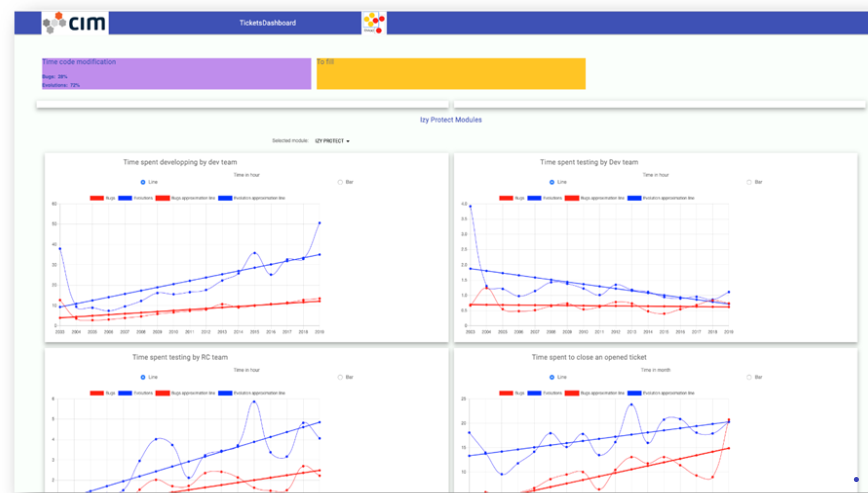
\includegraphics[width=\linewidth]{./figures/dashboard.png}
  \caption{Tableau de bord d'analyse de tickets 
}
  \label{fig:dashboardFig}
\end{center}
\vspace{-0.3cm}
\end{figure}
En me basant sur les résultats de \cite{Raja09}, j'ai utilisé la moyenne glissante avec une porté de cinq mois pour modéliser l'état du système.
La \figref{dashboardFig} présente un tableau de bord qui résume les resultats.

En effet, sur la \figref{dashboardFig} le premier graphe à gauche montre le temps nécessaire aux développeurs pour traiter les tickets. 
On voit que ce temps augmente.

Ceci pourrait être une conséquence de la complexité du code d'Izy Protect, ou bien, une mauvaise compréhension des besoins du client qui fait que le développeur prend du temps a comprendre le travail à faire.
Le premier graphe à droite  sur la \figref{dashboardFig} montre le temps des tests manuels du développeur. 
Contrairement au temps pour traiter les tickets, les développeurs passe de moins en moins de temps pour tester leur code.
Le deuxième graphe à gauche  sur la \figref{dashboardFig} montre le temps de test par l'équipe de ressource et qualité (RC). Ce temps augmente.
Ceci pourrait être dû  à la quantité de données traitées par les tests ou bien, la complexité d'Izy Protect qui peut être responsable de la complexité des cas de tests.
Le fait que les développpeurs testent de moins en moins Izy Protect  pourrait engendrer beaucoup de va-et-vient d'Izy Protect entre l'équipe de RC et des développeurs (le cercle -développement, RC: bugs, correction, RC )

Le deuxième graphe à droite montre le temps de fermeture de tickets. Ce temps est aussi en augmentation. 

Le tableau de bord se met à jour une fois par mois.
Donc je peux continuellement mesurer l'impact de l'utilisation des outils d'aide à la rétro-ingénierie que je proposerai.


% La  \figref{dashboardFig} présente quatre  
%  On peut remarquer une augmentation du temps passé par les développeurs pour traiter les évolutions ou les corrections.
%  De plus j'ai remarqué les courbes d'Izy Protect et de  son \textit{module Prestation} ont relativement les mêmes allures tout comme si tout le travail des développeurs ces dernières années n'est concentré que sur ce module-là.  
% Les données montrent aussi que les développeurs passes de moins en moins de temps à tester leur code. 

%======================================================================================================================
\subsection{Outil d'aide à la rétro-ingénierie logicielle}

Pour répondre aux exigences détaillées dans la  \secref{retroingenierie}, j'ai développé une suite d'outils d'aide à la rétro-ingénierie.
Ces outils sont développés au-dessus de la plateforme Moose \cite{Nier05c}.
En effet, la plate-forme offre un métamodèle générique et quatre outils principaux pour l'analyse des systèmes logiciels.
Il s'agit de (1) Famix : un meta-modèle qui permet aux développeurs de représenter un programme, (2) Moose Query: un API pour naviguer dans un modèle Famix,
(3) Les tags : utilisés pour enrichir le modèle de l'application avec des informations qui ne peuvent pas être directement déduites du code source et 
(4) Roassal : un framework de visualisation intégré dans Moose.

Dans la suite, je présenterai d'abord l'architecture mise en place pour les outils puis chaque outil.

\subsubsection{Architecture des outils }
\begin{figure}[htbp]
  \begin{center}
  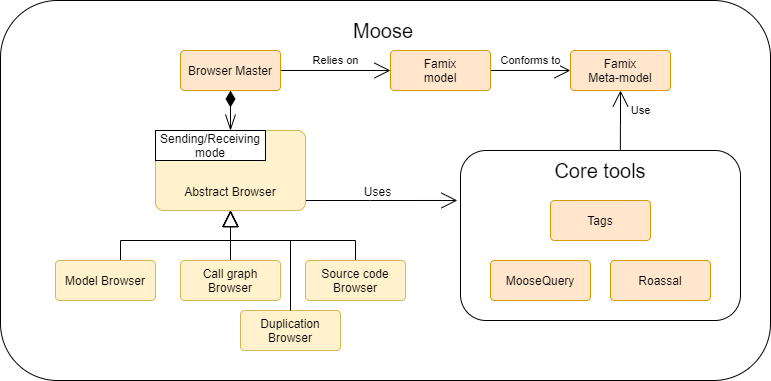
\includegraphics[width=0.8\linewidth]{./figures/architecture.png}
  \caption{Architecture de la suite d'outils}
  \label{fig:applicationArchitecture}
  \end{center}
  \vspace{-0.3cm}
\end{figure}

La \figref{applicationArchitecture} montre l'architecture globale de la suite d'outils.
L'architecture globale de la suite d'outils est principalement composée d'un \browserMaster et des navigateurs.
Le tout s'exécute sur une instance d'un modèle Famix. 
Il a été pensé dans le but de faciliter l'expérience du développeur dans les différentes activités de la rétro-ingénierie logiciel.
Le \browserMaster est responsable de l'échange d'information entre les navigateurs.
Il est au courant de tous les navigateurs ouverts. 
Il se charge de notifier tous les navigateurs ouverts en cas d'événement.

Tous les navigateurs partagent le même contexte. Quand une entité est selectionnée, chaque navigateur la montre de son propre point de vue.


% Chaque navigateur fonctionne sur une entité du modèle  local à lui.
% Cette entité peut être une seule entité ou un groupe d'entités.
% Il peut émettre ou recevoir un événement.
% Tous les navigateurs présentent un bouton qui indique son mode d'émission d'événement, et trois boutons qui indiquent son mode de réception d'événement (\eg \figref{graphAppel}).

% L'émission d'un événement par un navigateur est régie par son mode de propagation.
% En mode de propagation active, le navigateur émet un événement pour publier son entité courante à chaque fois que l'entité change.
% Dans le contraire, l'entité courante est gardée localement.

% Le comportement d'un navigateur à la réception d'un événement dépend du mode de réception de ce dernier.
% Ainsi, chaque navigateur possède trois modes de réception d'événement.  
% Il s'agit des modes (1) \textit{follow}: le navigateur  remplace son entité courante par l'entité reçue via l'événement.
% (2) \textit{highlight}: le navigateur cherche l'entité reçue via l'événement dans son entité courante, s'il la trouve, il la colorie.
% (3) \textit{ignore}: le navigateur ne fait rien à la réception de l'événement.

% %=============================================================================================================================
% \subsubsection{Nivigateur de modèle}
% \label{sec:navigateurModel}
% \begin{figure}[htbp]
%   \begin{center}
%   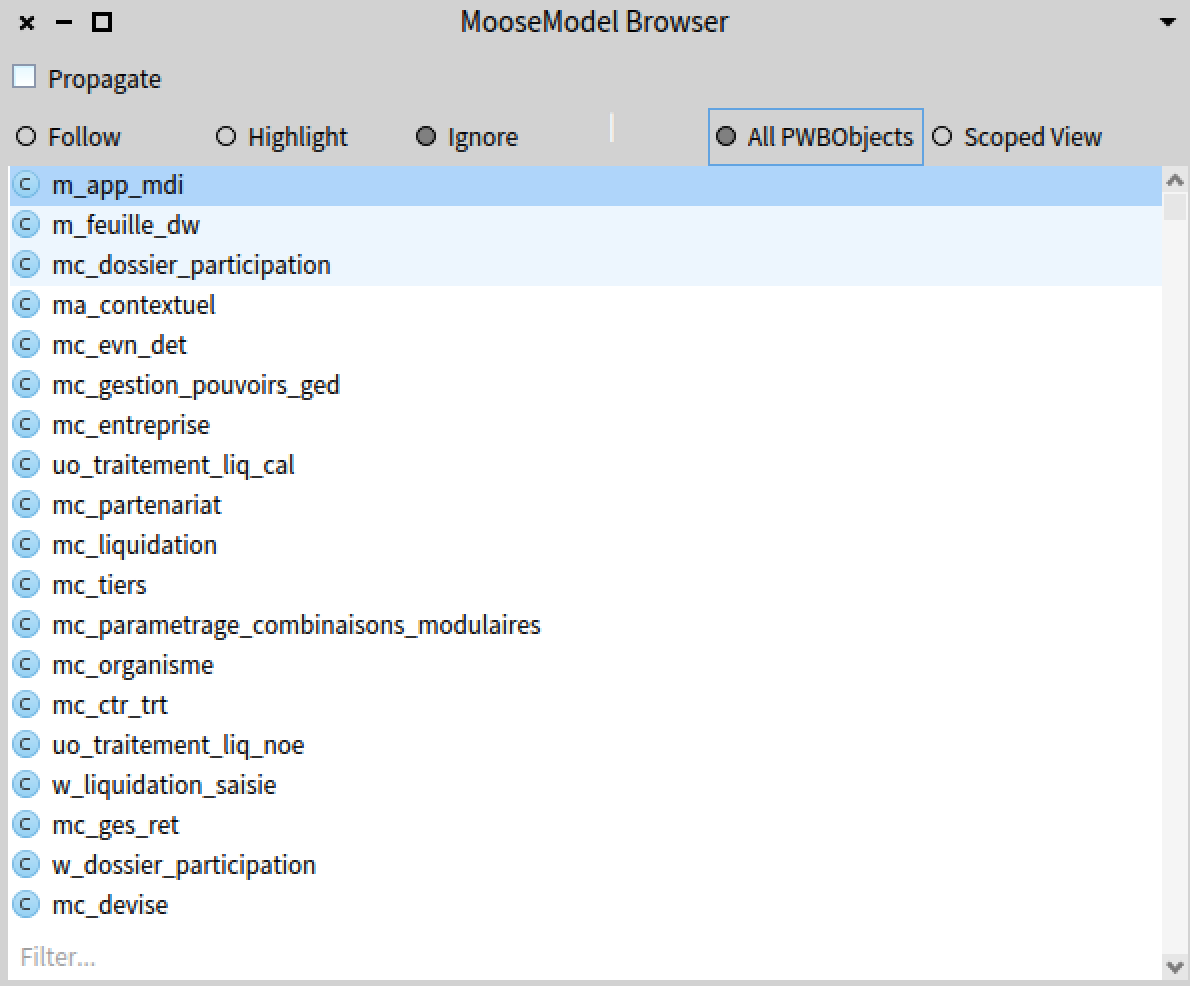
\includegraphics[width=0.6\textwidth]{./figures/modelBrowser.png}
%   \caption{Navigateur de modèle}
%   \label{fig:modelBrowser}
% \end{center}
% \vspace{-0.3cm}
% \end{figure}
% Le navigateur de modèle comme la montre la \figref{modelBrowser} outre la partie commune à tous les navigateurs, comporte deux boutons (\textit{All PWBObjects}, \textit{Scoped View}), un contenu et un champ de recherche.

% Le contenu navigateur présente par défaut la liste des entités que contient l'entité courante du navigateur. 
% L'utilisateur peut décider de se concentrer sur un certain nombre d'entités. Dans ce cas, il les sélectionne et il active le bouton \textit{Scoped View}.
% Pour le moment le navigateur de modèle est juste une liste. Mais il est prévu de l'étendre.

% Le champ de recherche du navigateur permet à l'utilisateur d'écrire une requête de recherche sur son entité Famix courante.
% Cette entité est pour la plupart du temps un groupe d'entité Famix.
% Cette requête peut être lexicale, sous forme de simple chaîne pour une recherche lexicale, ou structurelle.
% Par exemple, si l'utilisateur recherche \textit{include : FamixPWBAttribute}, le résultat sera toutes les entités contenant des FamixPWBAttribute (attributs PowerBuilder).

%================================================================================================================
\subsubsection{Navigateur de graphe d'appel}
\label{sec:callGraphBrowser}
\begin{figure}[htbp]
  \begin{center}
  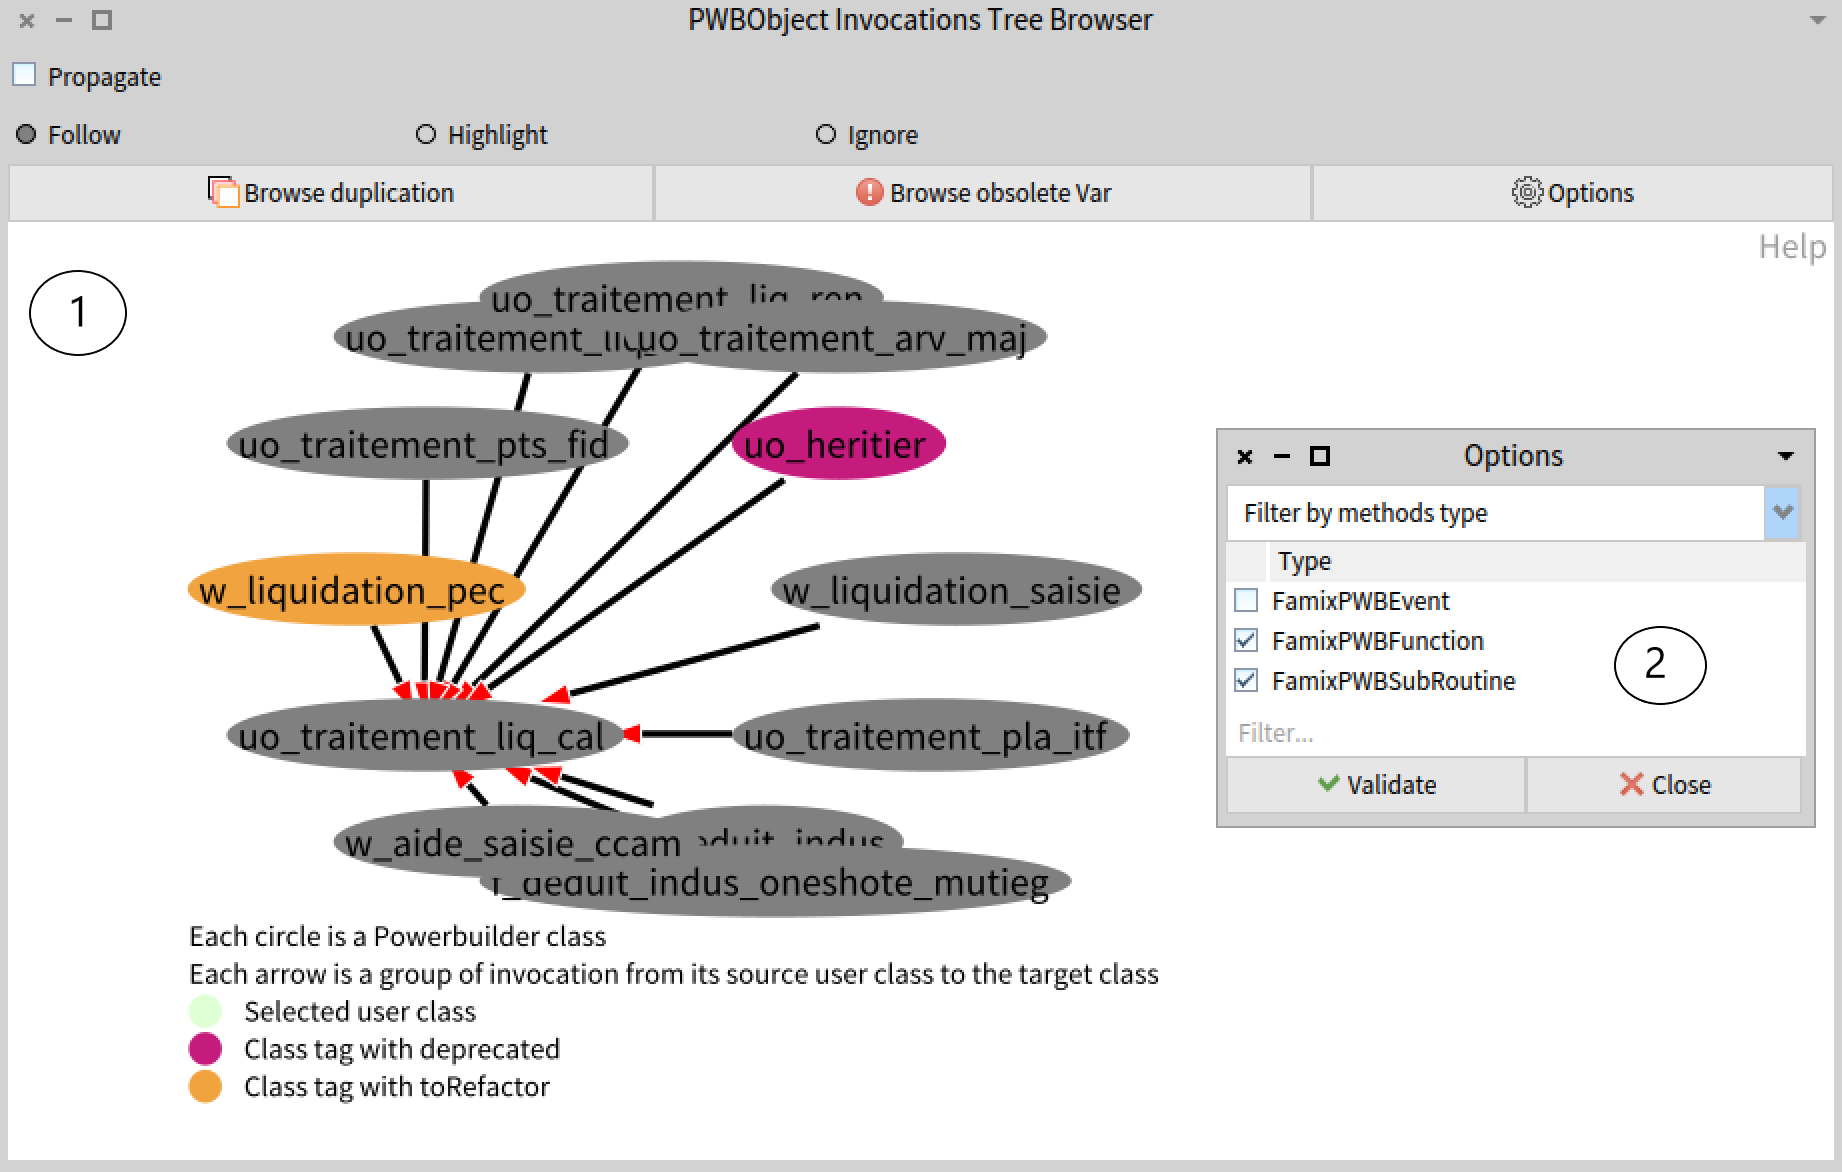
\includegraphics[width=0.9\textwidth]{./figures/callGraphBrowser.png}
  \caption{Graphe d'appel avec l'option de reduction de complexité du graphe}
  \label{fig:graphAppel}
\end{center}
\vspace{-0.3cm}
\end{figure}
La \figref{graphAppel} donne un aperçu du graphe d'appel avec les options.  
La fenêtre (1) de cet outil permet principalement de visualiser sous forme d'un graphe les entités qui utilisent l'entité courante du navigateur.
Les nœuds représentent les entités. Les flèches représentent l'ensemble des dépendances entre deux entités.
Le sens de la flèche indique le sens des dépendances.
En effet pour un système logiciel comme Izy Protect par exemple, ce graphe peut rapidement devenir illisible. 
Pour palier à ce problème, l'outil intègre un panel d'option (la fenêtre (2) de la \figref{graphAppel}) qui permet de filtrer le graphe par type d'entité à l'origine des appels.
Afin de donner plus de contexte aux développeurs, quand il glisse la souris sur une flèche, un pop-up lui montre le code source de toutes les dépendances que la flèche regroupe.

Le navigateur de graphe d'appel permet aussi aux développeurs de marquer les entités afin de leurs ajouter une information qu'on ne peut pas extraire directement du code source.
Une connaissance qui ressort de l'expérience du développeur sur le système.

\subsubsection{Navigateur de Code mort}

\begin{figure}[htbp]
  \begin{center}
  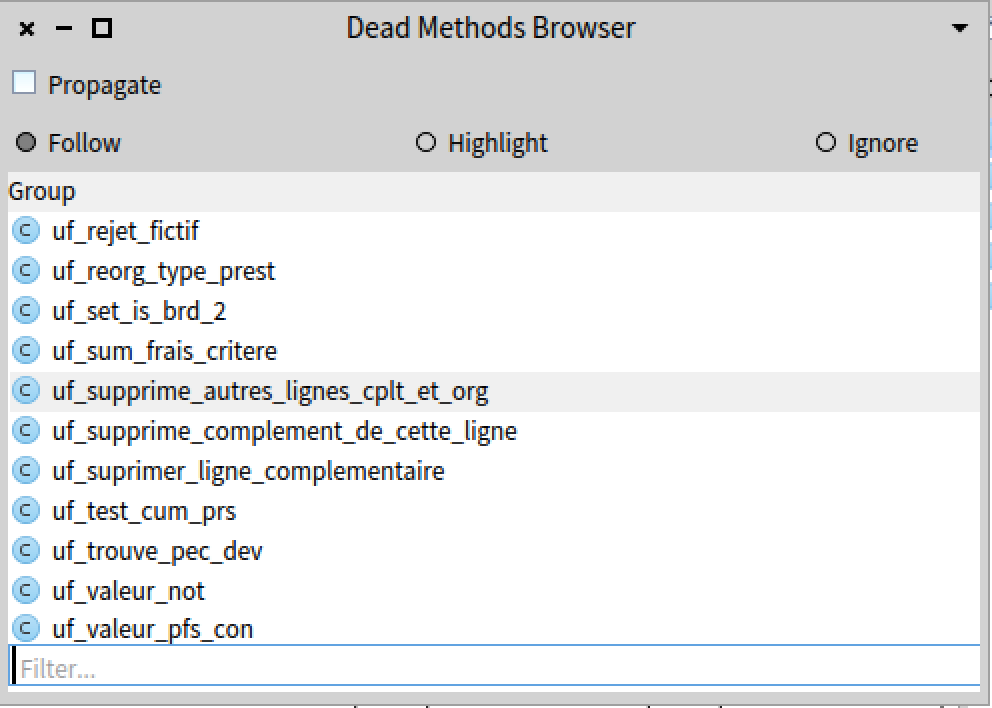
\includegraphics[width=0.5\textwidth]{./figures/deadMethodBrowser.png}
  \caption{Navigateur de code mort}
  \label{fig:deadMethodBrowser}
\end{center}
\vspace{-0.3cm}
\end{figure}
Un code mort est une partie du code source du programme qui n'est jamais utilisée lors de l'exécution de ce dernier.
Il peut être un obstacle à la compréhension d'un programme dans les activités de réto-ingénieries \cite{Wang17a}.
Malheureusement le code mort est identifié pour être généralement présent dans les logiciels \cite{Roma18}. 
Par conséquent, Izy Protect contient probablement de code mort.
Pour faciliter la compréhension de Izy Protect, il faut donc lister et enlever du  code mort .
La \figref{deadMethodBrowser} montre le navigateur de code mort.
C'est l'outil que je propose pour aider les développeurs à enlever le code mort.
Ce navigateur présent pour le moment les méthodes de l'entité courante du navigateur qui ne sont jamais appelées dans le système ainsi que les méthodes qu'elles appellent.

\subsubsection{Navigateur de code dupliqué}
\begin{figure}[htbp]
  \begin{center}
  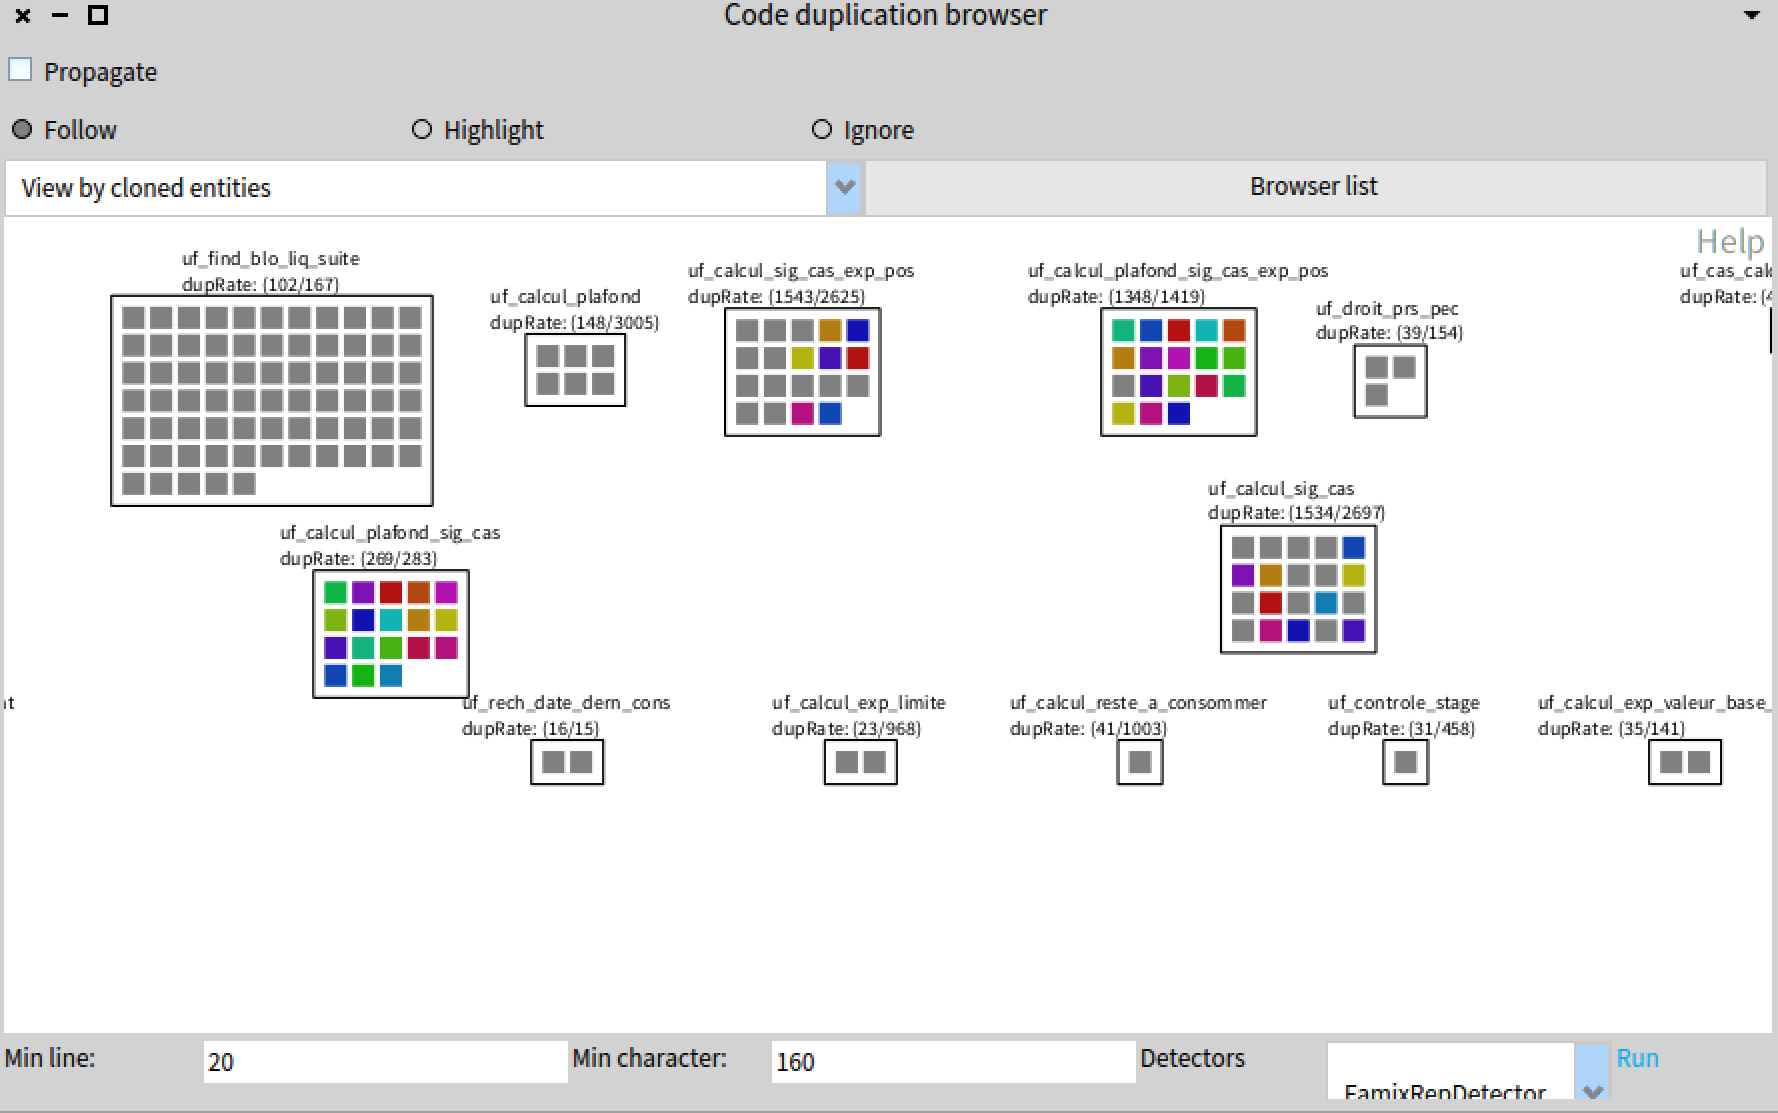
\includegraphics[width=0.9\textwidth]{./figures/duplicationBrowser.png}
  \caption{Navigateur de code dupliqué}
  \label{fig:duplicationBrowser}
\end{center}
\vspace{-0.3cm}
\end{figure}
D'après la littérature, (5-10\%) du code source des programmes de grande taille sont des clones \cite{Baxt98a}.
Détecter et enlever ces clones réduit le coût de maintenance de ces systèmes \cite{Baxt98a}.
Dans le contexte d'Izy Protect, pour la migration de sa partie métier, le fait de connaître les clones facilitera la migration dans le sens où les développeurs pourront migrer seulement une fois les clones ou bien le remettre facilement.
La \figref{duplicationBrowser} présente le navigateur de code dupliqué.
Les carrés externes représentent les entités qui contiennent des clones.
Dans le cas de la \figref{duplicationBrowser}, ces entités sont des  méthodes. 
Les carrés internes représentent les clones que présente une entité.
Les clones sont représentés de telle façon que l'utilisateur puisse facilement les inspecter.
Le navigateur de code dupliqué utilise actuellement un algorithme de détection basé sur l'égalité stricte des chaînes de caractères \citep{Duca99b}. 
Cet algorithme peut être remplacé par un algorithme plus sophistiqué pour détecter les doublons \citep{Roy07a}. 

Sur la \figref{duplicationBrowser}, la troisième entité sur la première ligne ($uf\_calcul\_sig\_cas\_exp\_pos$) et la deuxème entité sur la deuxième ligne ($uf\_calcul\_sig\_cas$) ont du code dupliqué entre eux.
Quand l'utilisateur clique sur $uf\_calcul\_sig\_cas\_exp\_pos$, ces clones (carrées internes) prennent des couleurs différentes.
Les clones que $uf\_calcul\_sig\_cas\_exp\_pos$ a en commun avec $uf\_calcul\_sig\_cas$, dans $uf\_calcul\_sig\_cas$ prennent les mêmes couleurs que leurs semblables dans $uf\_calcul\_sig\_cas\_exp\_pos$.
Par exemple le carré bleu dans $uf\_calcul\_sig\_cas$ a pris la couleur du carré bleu  dans $uf\_calcul\_sig\_cas\_exp\_pos$
parceque les deux carrées représentent le même fragment de code.  
Cela permet de voir plus facilement quelles entités ont des clones et de comparer les codes sources dans le navigateur de code que je présenterai dans la suite. 

%==========================================================================================================================
\subsubsection{Navigateur de code source}
\begin{figure}[htbp]
  \begin{center}
  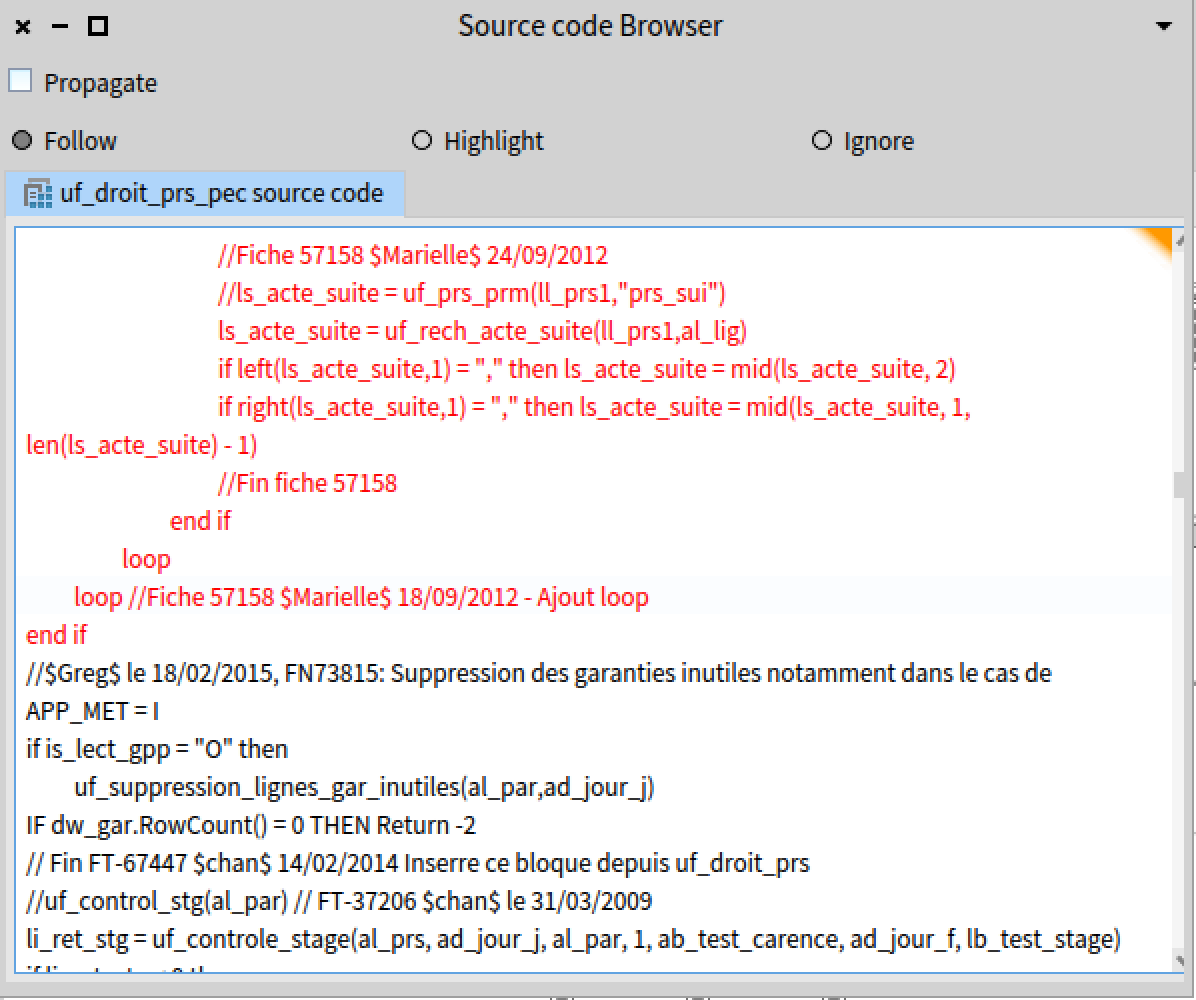
\includegraphics[width=0.7\textwidth]{./figures/sourceCodeBrowser.png}
  \caption{Navigateur de code dupliqué}
  \label{fig:sourceCodeBrowser}
\end{center}
\vspace{-0.3cm}
\end{figure}
La \figref{sourceCodeBrowser} présente le navigateur de code source. 
Ce navigateur est une fenêtre qui affiche le code source de l'entité courante.
En particulier dans le cadre d'un fragment dupliqué, le code source de l'entité qui contient ce fragment est affiché avec la partie du code qui représente le fragment dupliqué  en rouge comme sur la \figref{sourceCodeBrowser}.



% %================================================================================================================================================
 \subsubsection{Conformité des navigateurs par rapport aux critères des outils de rétro-ingénieurie}
J'ai construit les  navigateurs de façon a ce qu'ils respectent les critères précités dans la \secref{retroingenierie}.
En effet, l'environnement Moose offre les propriétés de \textbf{scalablilité}, \textbf{d'interopérabilité} \cite{Duca05a} dont héritent les outils. 
À travers les différentes réunions de présentations des outils aux développeurs, j'ai pris en compte  leurs critiques  afin que les outils non seulement, répondent à leurs besoins, mais aussi, soient facile d'utilisation et d'apprentissage.
 Le \textit{Navigateur de graphe d'appel} \secref{callGraphBrowser} répond aux critères  \textbf{d'abstraction} car il permet par exemple d'abstraire l'ensemble des invocations des méthodes d'une classe au niveau de la classe .
 


% %===============================================================================================================================

\section{Travaux futurs}
\label{sec:roadmap}
Tous les outils présents ci-dessus sont conçus dans le but de nettoyer le code et de visualiser les interactions entre les différentes classes d'Izy Protect.
%Par contre les développeurs ne les utilisent pas encore dans leur quotidien.
Pour vérifier que  les modifications n'introduisent pas d'erreurs, j'envisage de mettre en place les tests automatisés avec PBUnit. 
Ceci m'amènera à étudier les différentes approches de tests abordés dans la littérature afin d'identifier une approche qui s'adapte au contexte d'Izy Protect. 
Toutefois je pense que transformer les tests de données énoncés dans la \secref{izyProtect} en tests automatisés sera un point de départ. 

L'entreprise prévoit de migrer une partie du système dans une architecture orienté service. 
Les développeurs ont donc exprimé le besoin d'extraire des logiques métiers du code.
Plusieurs travaux sont présentés dans la littérature dans ce sens  notamment \cite{Lei05a,Cose12a,Norm12a} qui se basent sur l'analyse statique des interactions des fonctions avec les variables pour extraire les logiques metiers d'un système patrimonial. 
Je souhaite combiner cette méthode avec la méthode proposée \cite{anqu19a} pour proposer un outil d'extraction des logiques métiers dans les systèmes patrimoniaux.
Pour mener à bien la migration, je proposerai un outil de génération de tests unitaires automatisés pour les parties de Izy Protect concernées.
%Je mettrai en place et j'étudierai l'impact du DevOps à la CIM. 

\section{Publications}
Dans le cadre de cette thèse,
\begin{itemize}
\item l'article: \textit{Improving practices in a medium French company : First step} (\citet{Houe20a}) a été soumis
\item l'article: \textit{Towards a Versatile Reverse Engineering Tool Suite}  ( \citet{Houe20b}) a été accepté en version court.
\end{itemize}



\section{Formations}
Pour les formations doctorales, je cumule un  total de 41 crédits sur les 40 cédits minimums demandés pour une thèse CIFRE. 
Voici la liste des formations auquelles j'ai assistées  avec leurs crédits.
\begin{itemize}
\item Les fondamentaux du management d’équipe Session 1 (Ecole doctorale: 7 crédits) 
\item Gestion de conflit (CIM) 
\item Formation Propriété intellectuelle au service des doctorants tronc commun (Ecole doctorale: 10 crédits)
\item Intelligence économique et dynamique de l'innovation (Ecole doctorale: 10 crédits)
\item Communiquer en Anglais - Niveau confirmé - Stage intensif (Ecole doctorale: 14 crédits)
\end{itemize}
Bien que j'ai cumulé le nombre de crédits minimums demandés, j'assisterai à d'autres formations ayant trait avec le développement personnel. 
Car c'est sujet qui m'intérresse.
\section{Projet professionnel}
En ce qui concerne mon projet professionnel, je souhaite continuer dans l'enseignement supérieur : donner des cours et continuer dans la recherche.
Je pense que  la réingénierie des systèmes logiciels est un axe de recherche où beaucoup de travaux intéressant sont menés. Néanmoins il reste à faire et je souhaite contribuer à cela.
Toutefois, je ne me refuse pas l'idée de démarrer une start-up à l'issue de ma thèse ou travailler dans une entreprise.

\footnotesize{
  %\bibliographystyle{alpha}
  % natbib 
 \bibliographystyle{plainnat}
\bibliography{rmod,others,nextPubli}
}

\end{document}